\chapter{模型}
在文献中,源词和目标词分别被称为模型的输入和输出。源词通常可以用分布式表示来表示,称为输入词嵌入(Word Embedding),可以使用基于外部语料库的连续词袋模型或Skipgram模型来训练。而这两个模型来源于语言模型任务,并且为了在特征空间中产生可能的嵌入分布而被大大简化。另外,输出字通常表示为字索引(Indexing)或1-K编码,并且可以与softmax概率函数直接关联。

在本节中,我们将这个目标词表示扩展到一个分层的形式,使它们适配基于类和基于树的分层概率计算。首先,我们提出了一个在分层结构上建模参数的字编码方案。因此,考虑到GPU上的并行吞吐性能,我们推导出紧凑的代价函数及其梯度。同时,类或树上的单词分布对其性能有很大的影响,应该在训练阶段之前定义,这些动态交换算法在训练过程中改变了单词群或子树结构在这个研究中。我们采用了几个分层聚类和词汇分割策略,用统计,句法和语义知识来初始化其结构,以达到一个稳定和可以预期的性能。而且,在推理过程中,不同于传统的softmax情况,得到最好的候选者自然是可行的,层次推理不能直接用 softmax 方法来实现。我们讨论基于树和基于类的搜索策略的两种不同的推理情况:a)打分:输出给定序列的概率;b)排序   :在给定的上下文中获取得分最高的一个候选单词。
\section{模型一}
\subsection{基于二叉树的单词编码}
在叶子上有文字的二叉树的情况下,我们可以通过访问从根到叶的所有内部节点来定位每个特定的词。在这里,单词$ w $的路由表示所有内部节点$ \theta^w_i $和它访问的边缘$ d ^ w_i $。

为了说明,$ \theta_i ^ w $表示到达单词$w$的路径上的$ i^{th} $层上的非叶节点,并且$\mathbb{R}^m $中的$ \theta_i ^ w$ 其中$ i \in [0, l ^ w - 1] $。同样,$ d_i ^ w $表示连接$(i-1)^ {th} $和$ i ^ {th} $层节点的边。对于每个非叶子节点,向下移动到左边的分支标记为$ -1 $,选择正确的分支标记为$ + 1 $。因此,在$i\in[0,l^w-1]$, $d_i^w\in \{-1,+1\}$。 此外, $l^w\approx \log \mathcal{|V|}$~表示从根到叶单词的路径长度。通过这个方案,我们可以通过表示极性路径来定位每个单词,将单词索引或单热表示改变为单词极性编码元组$(d ^ w,\theta ^ w)$。


在实现过程中,我们维护一个路径查找表$ \Gamma $,记住每个单词$ w $从根到叶的所有访问内部节点的索引。这样,通过从$ \Gamma(w)$中选择所有节点,从参数矩阵${\Theta} $中检索$ \theta ^ w $。由于${\Theta} $的第一维是:
\begin{equation}\label{equ:sums}
\sum_{i=0}^{\log \mathcal{|V|}}{2^i} = \mathcal{|V|} -1.
\end{equation}
因此,p-tHSM模型没有增加模型参数。

此外,通过从矩阵$\mathcal{D}$中获得$w^{th} $行向量来检索$d^w$,其中$w$是词汇表中的单词索引。 此外,$\{\Gamma,\mathcal{D}\}$ 是由层次聚类算法定义的,$\Theta$是通过训练数据集上的梯度下降来优化的。为了清楚起见,$ \Theta $是模型的参数,$ \Gamma $记忆路径节点索引信息,$\mathcal {D}$取 $ \{ - 1,+1 \} $中的值。

如图~\ref{fig:tree_hsm}~所示,内部参数 $\theta_i^w$, 边 $d_i^w$ 并且单词在树的叶子节点上. 除此之外, 加粗的那条路径从根节点到叶子节点 $w$ 被定义为参数对 $(d^w,\theta^w)$。其中 $d^w$ 是一个向量, $\theta^w$ 是一个参数矩阵. 例如, $d^w=[-1,+1,-1]$ , $d^{v}=[-1,+1,+1]$。
\begin{figure}[!h]
  \centering
    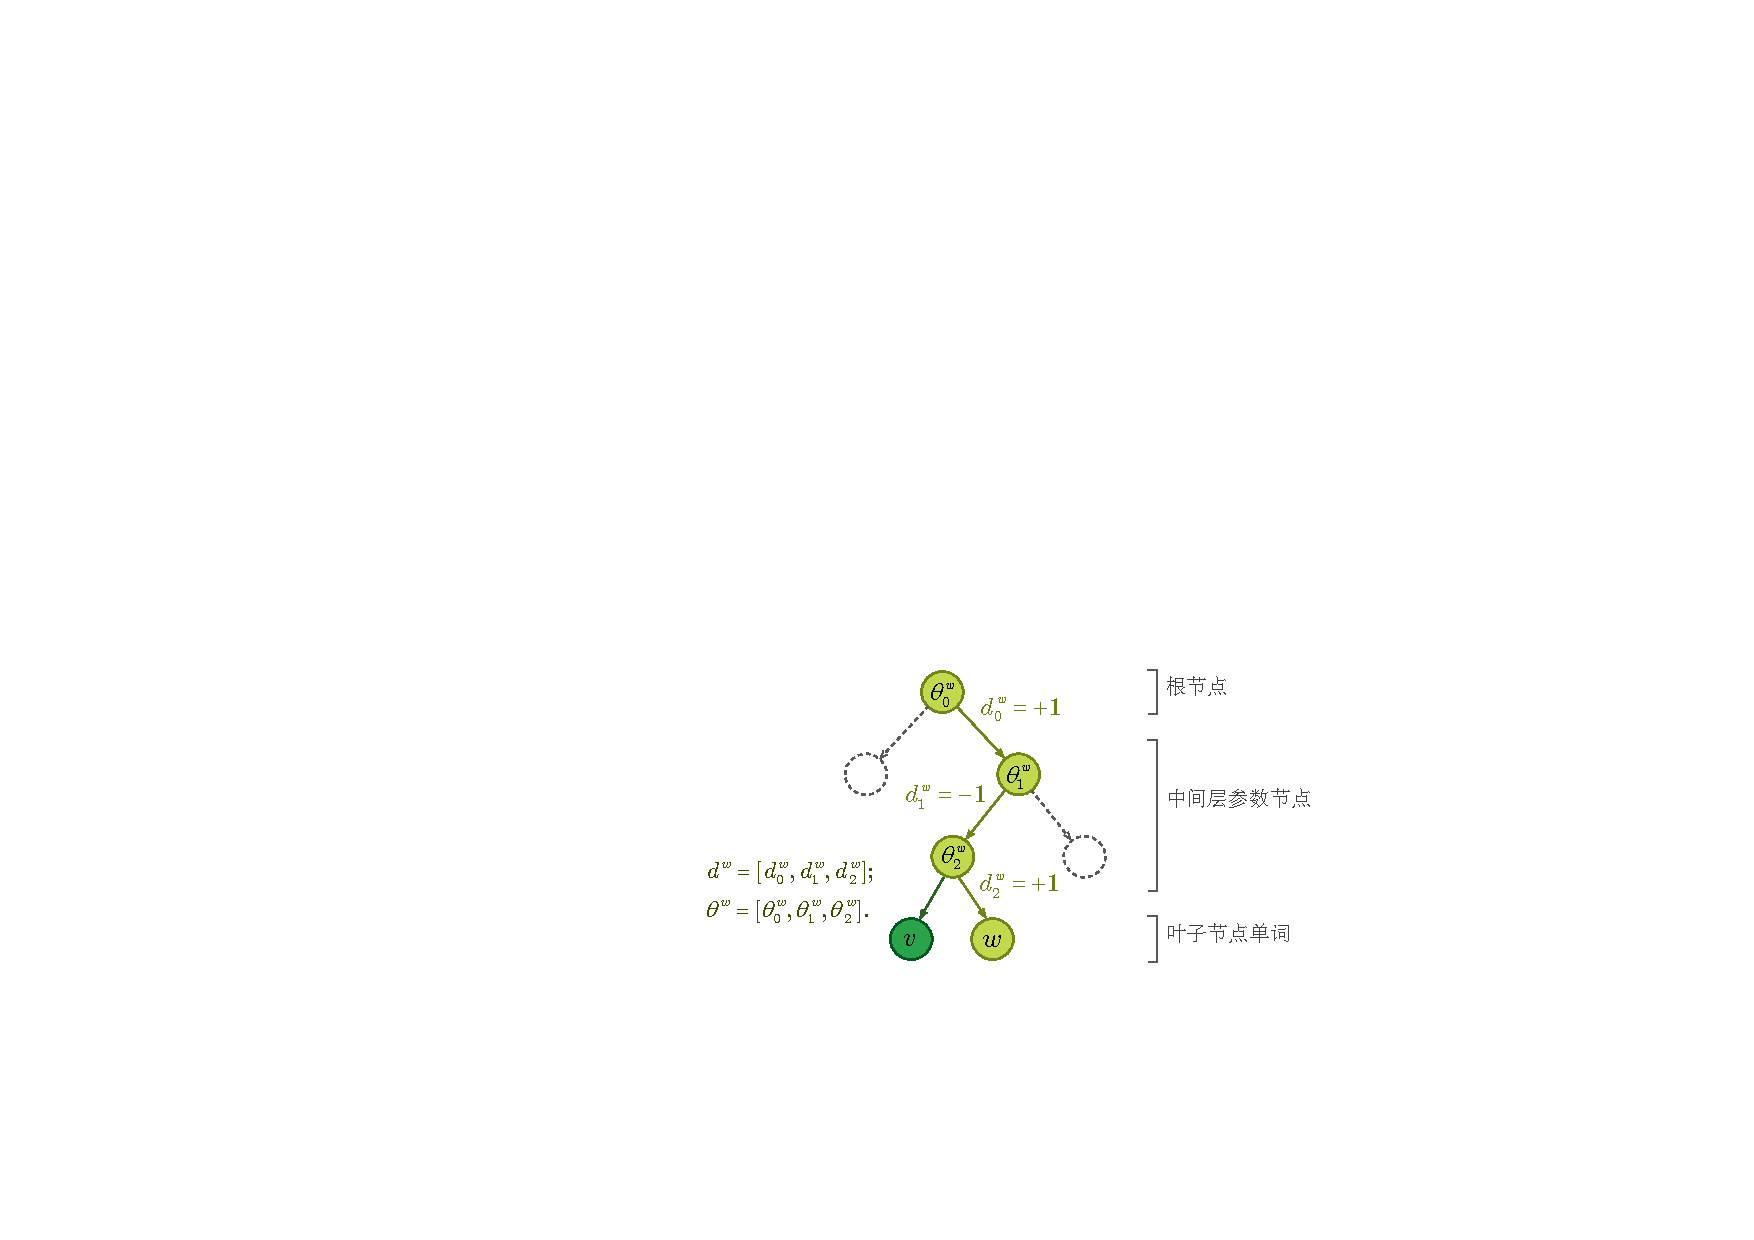
\includegraphics[width=0.75\linewidth]{./figures/thsm.pdf}
\caption{树状层次概率模型}\label{fig:tree_hsm} %
\end{figure}

\subsection{基于二叉树的代价函数和导数}
 \begin{equation}
p(d^w_i|\theta_{i}^w,h) =\sigma(\theta_{i}^w h)^{d_i^w}\times[1-\sigma(\theta_{i}^w h)]^{1-{d_i^w}},d_i^w \in [0,1]
\end{equation}
 \begin{equation}
p(d^w_i|\theta_{i}^w,h) =\sigma(\theta_{i}^w h)^{d_i^w}, d_i^w \in [-1,1]
\end{equation}
\begin{equation}
p(d^w_i=\pm 1|\theta_{i}^w,h) = \sigma({d_i^w}\theta_{i}^w h)
\end{equation}

一个单词的概率 $w$:
\begin{equation}\label{equ:pw}
\begin{split}
 \log p(w|h)=&\log\prod_{i=0}^{l^w-1} p(d^w_i|\theta_{i}^w,h) = \sum_{i=0}^{l^w -1} \log\sigma(d_i^w \theta_{i}^w h)\\
 =&\log\sigma({d^w}^\top \theta^w h)=\zeta(- {d^w}^\top \theta^w h )
 \end{split}
\end{equation}
其中 $\zeta(z)$ 代表 softplus 函数: $\zeta(z)= \log (1+\exp(z))$ 他的导数是 $\sigma$ 函数, 其导数公式是: ${\mathrm{d}\zeta(z)}/{\mathrm{d} z}= \sigma(z)$~\upcite{DBLP:conf/nips/DugasBBNG00}. Minimising the tree-based negative log-likelihood is directly maximising softplus loss and the probability of estimated words.

Nonetheless, in the traditional tHSM algorithm, the model calculates the log-probability of every node layer-by-layer. Consequently, the overall joint log-probability of this word is summarised linearly through the layers. Thus the time complexity of tHSM takes $O(\mathcal{|H|\log|V|})$:
\begin{equation}
\ell(\theta|h,w) =\sum_{i=0}^{l^w-1} \{(1-d'^w_i)\log (\sigma(\theta_{i}^w h))  + {d'^w_i}\log (1-\sigma (\theta_{i}^w h))\}
\end{equation}
where $d'^w_i\in \{0,1\}$, and these two parts model the joint probability distribution of the left and right branch of internal nodes separatively.

Noticeably, the main difference between p-tHSM and tHSM is that: a) tHSM algorithm involves many tiny matrix multiplications, instead in p-tHSM we load all parameters $(d^w, \theta^w)$ directly as 1D vector and 2D matrix at the expense of runtime memory consumption and we consider the multiplications of this vector and giant matrix, as shown in Fig.~\ref{fig:tree_hsm}; b) A compact loss function of the model is deducted and the nodes' log-probability are calculated simultaneously which results in better time efficiency for p-tHSM model.

As a consequence, the model's parameters $\{\theta^w,h\}$ are optimised with regard to its gradient.
\begin{equation}
\begin{split}
\frac{\partial \ell}{\partial \theta^w}=&(\sigma({d^w}^\top\theta^w h) -1){d^w}^\top h \\
\frac{\partial \ell}{\partial h}=&(\sigma({d^w}^\top \theta^w h) -1){d^w}^\top \theta
\end{split}
\end{equation}

\begin{figure}[!ht]
  \centering
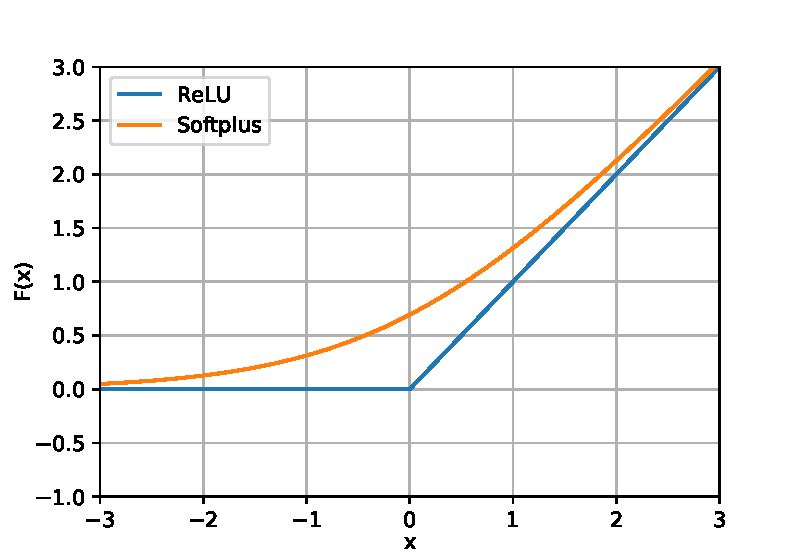
\includegraphics[width=0.45\linewidth]{./figures/relus.pdf}
\caption{Softplus和ReLU函数的示意图}\label{fig:soft}
\end{figure}

二叉树分解的一个主要优点是它避免了在整个词汇表中概率的归一化,因为树中词的汇总概率自然等于1。
\begin{equation}
\sum_{w\in \mathcal{V}}{p(w|h)}=\sum_{w \in \mathcal{V}}\sum_{i=0}^{l^w-1}{\sigma(d_i^w\theta_{i}^w h)}=1.
\end{equation}




\subsection{基于二叉树的推理算法}
考虑到本节开始提出的第一个问题,即给定序列$ [w_1,\ cdots,w_T] $的概率。 直观地说,当给定相应的上下文$ h $时,我们可以通过获取一个特定单词$ w $的概率或对数概率来分解问题:
\begin{equation}
\begin{split}
    p(w|h) =&\sigma({d^w}^\top \theta^w h)\\
   \log p(w|h) =& -\zeta(- {d^{w}}^\top \theta^{w} h )
\end{split}
\end{equation}
其中概率$ p(w | h)$和单词$ w $的对数概率$ \log p(w | h)$可以直接通过等式~\ref{equ:pw}和~\ref{equ:cost}分开。 因此,这个序列的概率可以形式化为:
\begin{equation}
\ell(\theta|h,w) =\sum_{i=0}^{l^w-1} (1-d'^w_i)\log (\sigma(\theta_{i}^w h))  + {d'^w_i}\log (1-\sigma (\theta_{i}^w h))
\end{equation}
显然,这种类型的操作比传统的softmax方法有效得多,它涉及$\mathcal{O}(\mathcal {| H | \log| V |})$计算。

关于第二种情况,当给定前一个上下文(也被称为$\arg\max $方法)时,在整个词汇表中搜索最可能的下一个话语单词。我们可以在选择最上面的一个候选人之前计算词汇表中所有单词的概率。这个过程仍然是昂贵而缓慢的,因为它涉及到整个词的分层树。如在算法~\ref{alog:argmax}中所描述的,为了避免两个小概率的精确度损失问题,计算每个内部节点的对数概率。

而不是搜索全局最优结果,我们可以用局部贪婪算法搜索次优结果。具体而言,对于$ i $ -th层中的节点,当$ p(d ^ w_i | \theta_{i} ^ w,h)\ge 0.5 $时选择左边的分支,相反适用,如算法~\ref{alog:greed_argmax}所示。因此,计算时间复杂度仍然是$ \mathcal{O}(| H | \log \mathcal {| V |})$。


\begin{algorithm}[!ht]
\SetAlgoLined
\KwData{隐藏层输出 $h$;}
\KwResult{ 预测的单词 $w$. }
 路径列表 $\mathtt{path}$=[] \;
\While(\tcp*[h]{逐层搜索}){$k \le \log \mathcal{V}$ }{
\eIf{$p(d_{k} |\theta_{k},h) \ge 0.5$ }{
 $k=  k*2$ \tcp*[r]{左分支}
}{
 $k = k*2+1$ \tcp*[r]{右分支}
}
 $\mathtt{path}$.append($k$) \tcp*[r]{append $k$ to path list}
}
 alter $\mathtt{path}$ with word $w$ by looking-up table $\Gamma$.\
 \Return $w$ \;
\caption{逐层贪心搜索 Argmax}\label{alog:greed_argmax}
\end{algorithm}

\subsection{基于二叉树的聚类算法}
词汇表中每个单词$(d^w,\ theta^w)$的极性编码与树的结构密切相关。对于提出的p-tHSM方法,我们采用了几种树聚类算法来提高其性能和稳定性。这些聚类算法为每个单词生成二进制前缀字符串,表示树中单词的位置,并将用于初始化p-tHSM方法。


1)\textit{Unigram 聚类}它根据词频对词汇进行排序,并根据单词统计从buttom到top进行合并,也称为Huffman Encoding~\upcite{DBLP:conf/nips/MikolovSCCD13}。

2)\textit{Bigram 聚类\footnote{https://github.com/percyliang/brown-cluster}}。它是一个层次凝聚聚类算法,使用bigram上下文来确定单词的分布相似性,将相似的单词放置在二叉树的附近位置~\upcite{DBLP:journals/coling/BrownPdLM92,liang2005semi}。在将簇大小指定为1之后,它从底部到顶部合并具有一个节点的单词。生成的单词二进制路由正是分层二进制结构的分布。

3)\textit{语义聚类\footnote{https://code.google.com/archive/p/word2vec/}。}在引导式的方式下,词嵌入在外部语料库上训练,我们将传统的凝聚式聚类应用于字嵌入特征~\upcite{DBLP:books/sp/mining12}。

\section{模型二}
\subsection{词表划分算法}
为了提高GPU架构的加速比,并支持广义的词汇分割方法,我们提出了一种基于类的分层softmax方法的高效通用结构。

扁平化的词汇表被分成类别向量$ \theta^c $和输出矩阵$ \theta^o $ 结构,其中前者定义了不同类别的概率$ p ^ c $,而后者则模拟了该分区组内的单词概率$ p ^ o $,如图~\ref {fig:chsm}所示。输出矩阵的维度是类维度和分组词维度。如果将词汇$ \mathcal {V} $划分为不等大小的组,我们首先将词组分类为等长矩阵,填充零掩码。对于不在这个组中的剩余节点,我们使用掩码向量$ \ theta ^ m $来消除其对概率计算和成本汇总过程的影响。因此,分组的文字尺寸是最大的组尺寸。如果我们应用相同大小的词汇分割算法,掩码向量$ \theta ^ m $可以被忽略,并且分组的词维度是$ \mathcal {| V | / | C |} $,其中$ \mathcal {| C |} $表示类维度。要注意的是,如果$ \mathcal {| V |} $不能被$ \mathcal {| C |} $整除,那么最后一组中的确切单词应该小于组大小。

更重要的是,我们将一次性索引设置分成一个元组$(w ^ c,w ^ o)$,可以从查找表$\Gamma $中检索给定单词索引$ w $。此外,$ w ^ c $指定类ID,$ w^c $表示该组内的本地单词索引。
\begin{equation}\label{equ:partition}
 \theta^m=
\begin{cases}
    \text{单位矩阵} ,& \text{若均匀划分} \\
    \text{掩码矩阵},   & \text{否则}
\end{cases}
\end{equation}


如图~\ref{fig:chsm}~所示,扁平化的词汇可以形成右上矩阵,矩阵的大小应该大于或等于词汇表,不需要外部掩码。
另外,拼合词汇可以形成左上矩阵,需要外部掩模,矩阵的构成依赖于分割算法。
\begin{figure}[!ht]
  \centering
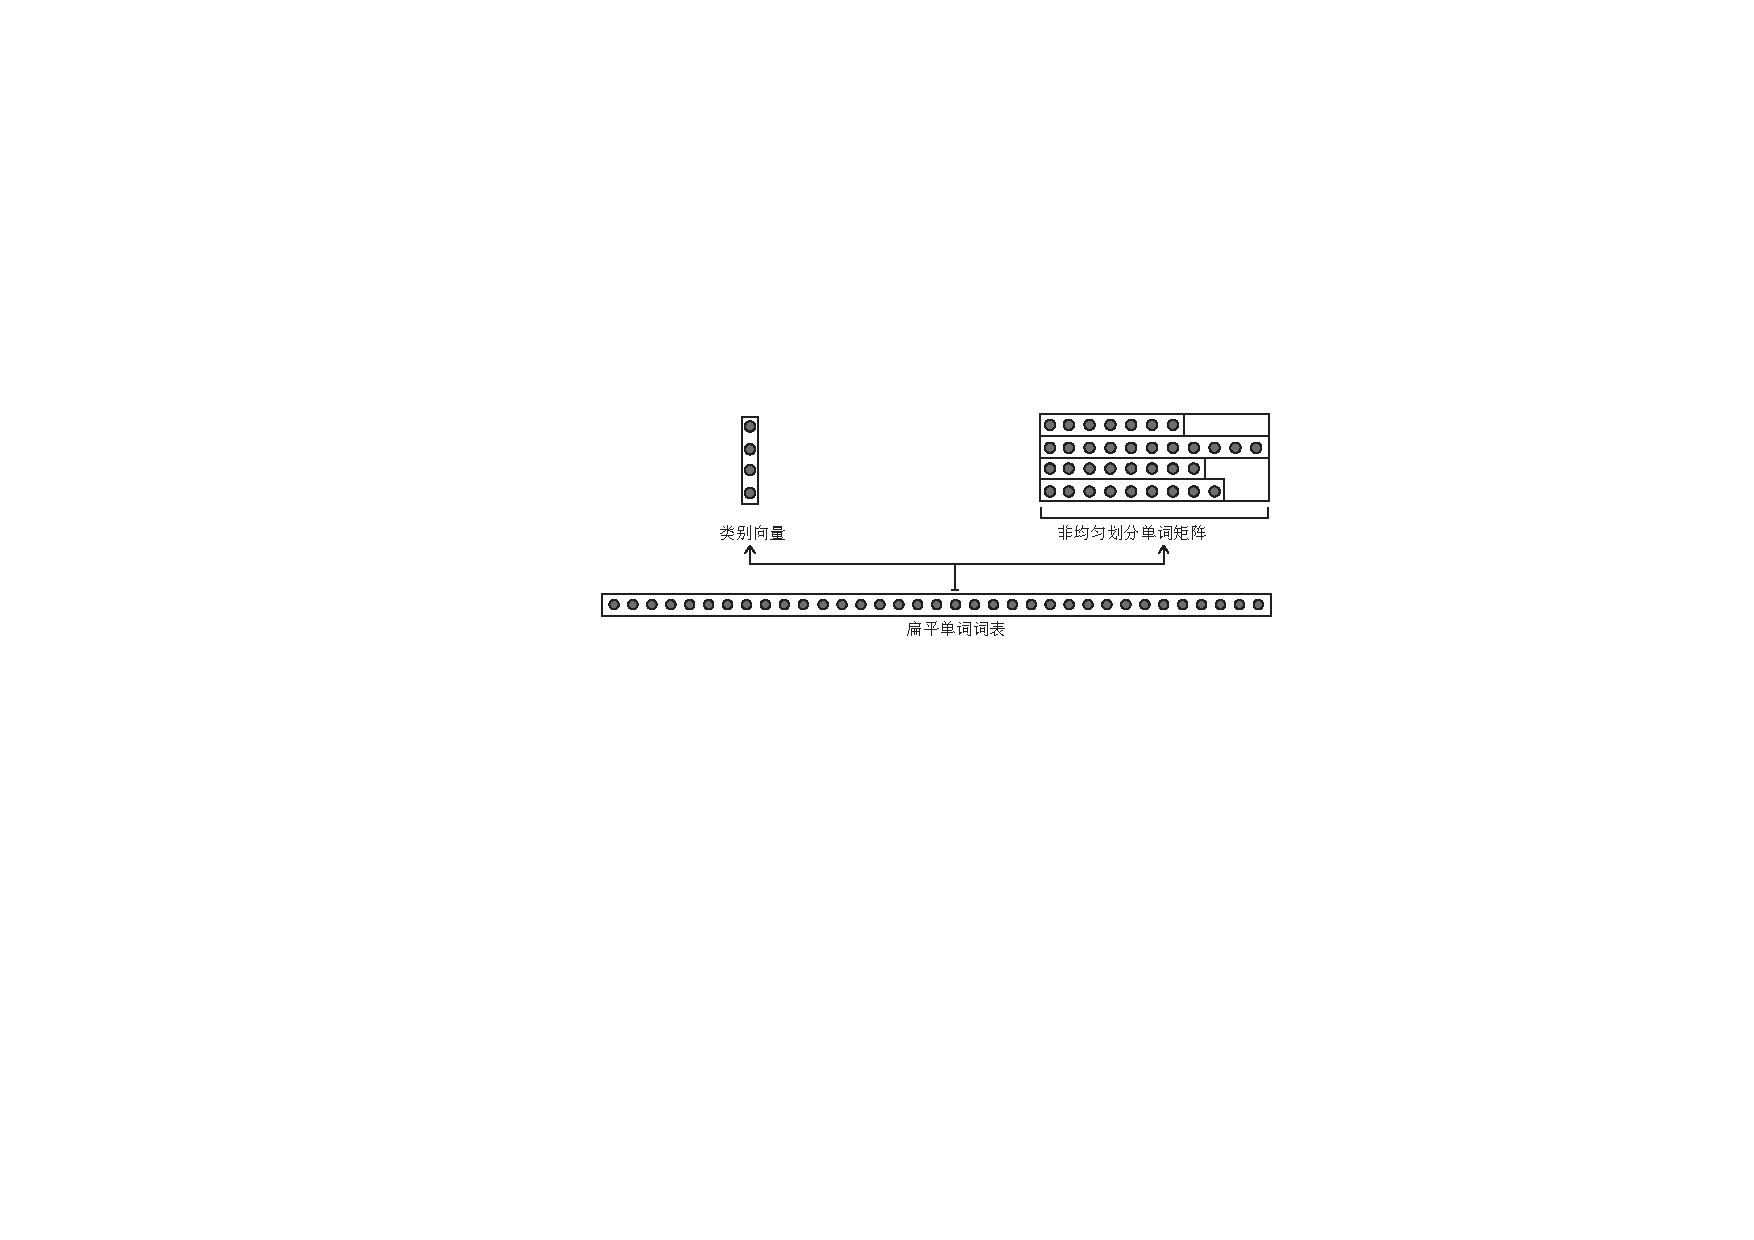
\includegraphics[width=0.85\linewidth]{./figures/chsm-simple.pdf}
\caption{cHSM算法的两种不同的词表划分算法}\label{fig:chsm}
\end{figure}


\subsection{基于类别的代价函数和导数}
给定最后一个隐藏层输出$ h $,那么这个分区组中的每个组和每个单词的概率可以被定义为:
\begin{equation}
\begin{split}
\log p^c(c|h) &= \theta^c h-\log \sum{\exp( \theta^c h )} \\
\log p^g(w|w^c,h)&=\theta^o h -\log\sum\exp{(\theta^o h)}
\end{split}
\end{equation}
其中$ p ^ c $和$ p ^ w $是分别计算而不是并行计算的,因为主要的计算瓶颈是局部标准化的单词概率$ p ^ w $,所以这两个概率的并行计算不会达到时间效率提升。


尽管如此,掩码矩阵不能直接应用于这个分词矩阵,应该应用在log softmax概率计算程序中。 为了说明,在softmax函数中:$ p(x_i)= {\exp({x_i}})/ {\sum_j \exp(x_j)} $,如果$ x_k = 0 $,但其概率$ p(x_k)> 0,\quad \exp(x_k)> 0 $。 因此,该组中确切的后验词对数概率计算如下:
\begin{equation}
  \log p^o(w|w^c,h)=\theta^o h -\log\sum\theta^m\exp(\theta^o h)
\end{equation}

那么,这个模型的损失函数可以形式化如下:
\begin{equation}
\ell(\theta|h) =\log p^c(w^c|h) +\log p^o(w^o|w^c,h)
\end{equation}
其中类别水平损失等于负对数似然的常见设置,并且字水平损失需要在计算其损失时指定其类别 $ w ^ c $。

在训练过程中,$ w ^ c $是预定义的,在测试过程中,$ w ^ c $由$ \arg\max_c p ^ c $获取。 类似地,关于梯度,模型的参数被优化。
\begin{equation}
\begin{split}
\frac{\partial \ell}{\partial \theta^c}=& (\delta_{ij}-p(c|h))h \\
\frac{\partial \ell}{\partial \theta^o}=&(\delta_{ij}-p(w|c,h))h \\
\frac{\partial \ell}{\partial h}=&(\delta_{ij}-p^c(c|h))\theta^c + (\delta_{ij}-p^o(w|c,h))\theta^o
\end{split}
\end{equation}

将词汇分成相互排斥的词组的一个主要优点是:a)避免了在整个词汇表上规范概率。 由于$ p ^ c $是在类维度上标准化的,$ p ^ o $是在最大组大小上进行标准化的。 所以在第二个方程中,多余的其他组被忽略,在最大的文本数据集中二者都不会超过1000。 b)与基于树的结构相比,它在词汇表上的分布更少,在分解步骤中丢失的信息更少。 c)与子字级方法相比,它不会增加序列长度,也不会影响复发性细胞的长程依赖性建模。



\subsection{基于类别的测试推理}
在推理阶段,对于cHSM模型来说,序列的概率评分要容易得多。
类似于以前的方法,我们可以通过重新研究我们的训练模型来解决第一个问题:
\begin{equation}\label{equ:class_inf}
   \log p(w_1,\cdots, w_T)=\sum_t^T\log p(w_t|h_t)=\sum_{t=1}^{T}\log p^c(w^c_t|h_t) +\log p^o(w^o_t|w^c_t,h_t)
\end{equation}
我们发现这种类型的操作比传统的softmax方法有效得多,该方法涉及$ \mathcal{O (| H | \sqrt{|V|} )}$计算。

其次,对于$\arg\max $的情况,我们可以在选择最佳候选项之前计算词汇表中所有单词的概率,这在直观上是正确的,但在计算上是昂贵的且慢,因为涉及到整个单词的分割矩阵。 此外,我们仍然可以在算法~\ref{alog:exact}~中对上述方法进行少量修改,然后计算确切的最高候选人。
\begin{algorithm}[!ht]
\caption{Exact $\arg\max$ algorithm for cHSM.}\label{alog:exact}
\KwData{ 隐藏层输出 $h$;}
\KwResult{ The predicted best candidate word $w$.}
 $\hat y^o=\arg\max_o{\log p^o(w| c,h)}$ \tcp*[r]{select best candidates in every group}
 $\tilde y^c=\arg\max_c{(\log p^c(y^c|h)+\log p^w(\hat y^w|\hat y^c,h))}$\tcp*[r]{calculate best candidate}
 alter $(\tilde y^c,\hat y^o[\tilde y^c])$ with word $w$ by looking-up table $\Gamma'$ \;
 \Return $w$ \;
\end{algorithm}

此外,cHSM算法的性能对分区算法有些敏感,因为某些方法可能会产生高度不平衡的字组,并且这种偏斜的分布会在算法中产生标签偏差问题。第一个本地 $\arg\max_o$ 进程~\upcite{DBLP:conf/icml/LaffertyMP01}。然而,在大多数情况下,如果选择合适的参数,则可以考虑不平衡的问题,本文考虑平衡词汇分区的广义形式。

为了说明,考虑两个类 $ c_p $ 和 $ c_q $,这两个类的容量是不同的,例如 $| c_p | \le | c_q |$。在计算了最后一个隐藏层输出 $h$与类图层参数的相似性之后,我们继续计算 $h$ 与每个组的内部单词 $w$ 的相似性得分,这些单词在每个特定组中都没有进行局部规范化整个词汇。当$ | c_p | \approx|c_q|$ 表示我们希望将词汇聚类成等大小的群组,而不是高度倾斜的群组分布时,可以减轻标签偏差问题,其中$ | c_p | \ll | c_q | $ 。更具体地说,对于分布不均的情况,对于类 $ c_q $中的单词来说这个概率被一大群单词稀释是不公平的,这样算法更有可能以较高的概率取出这个小组中的单词,放弃在其他大集团有更多的潜在的话。

我们可以用局部贪婪算法搜索次优结果,而不是搜索确切的全局最优结果,而是建议将这个$ \arg\max $进程分解为两个阶段:a)计算类概率,并剔除顶端一个$ \hat c $; b)计算该类别的单词概率$ \hat c $,并选择具有最高本地单词概率的单词。这个算法会给psudo最好的候选人,但是与原始算法~\ref{alog:exact}相比,它的运行速度要快得多。而且,由于分组词在本地进行归一化,标签偏差问题可以在一定程度上缓解。在实验研究中将讨论算法~\ref{alog:exact}和~\ref{alog:argmax}的详细不同性能。
\begin{algorithm}[!ht]
\KwData{隐藏层输出 $h$;}
\KwResult{ The predicted best candidate word $\hat w$.}
 $\hat w^c=\arg\max_c{\log p^c(c|h)}$ \tcp*[r]{select best candidate among classes}
 $\hat w^o=\arg\max_o{\log p^o(w|\hat w^c,h)}$\tcp*[r]{select best candidate in specific group}
 alter $(\hat w^c,\hat w^o)$ with word $\hat w$ by looking-up table $\Gamma'$ \;
 \Return $\hat w$
 \caption{Psudo $\arg\max$ algorithm for cHSM.}\label{alog:argmax}
\end{algorithm}

\subsection{词表划分算法}
由于cHSM模型的性能与其词汇分割算法密切相关,我们将聚类算法的现有工作进行汇总,并将可能的方法分类如下:

1)\textit{随机初始化} 这种直观的方法忽略了单词的所有外部信息,因此单词与随机随机播放过程是等分的。这是揭示其他聚类方法下界的最坏情况,也可以揭示应用高级聚类策略的相对收益。

2)\textit{字母顺序} 这种方法根据字符级别的信息对单词进行排序,同一组中的单词共享一个相似的子字符串。

3)\textit{Unigram 聚类}这些单词首先根据它们在文本中的频率排序,然后通过放置边界使得每个类别占总概率质量的恒定部分,从而形成连续单词块。这种方法具有这样的性质:较低编号的类比较高编号的类具有更少的成员,因为它们的成员更频繁~\upcite{DBLP:conf/nips/MikolovSCCD13}。

4)\textit{Bigram聚类}。它是指布朗聚类方法,这是历史适用于基于n-gram的基于类的模型~\upcite{DBLP:journals/coling/BrownPdLM92,liang2005semi}。单词使用相同的bigram上下文分组到相同的行中。

5)\textit{结构聚类\footnote{https://github.com/AlonDaks/unsupervised-authorial-clustering}。}根据文本中的词性和句法结构划分词汇~\upcite{daks2016unsupervised} 。

4)\textit{语义聚类。}我们将传统的kmeans聚类方法应用到预训练的词嵌入,使得我们可以通过指定聚类的大小将词汇分成不同的形状。
\section{本章小结}